% !TeX root = ../main.tex
\section{Experiments}
\label{sec:experiments}

\subsection{Experimental Setup}
\label{subsec:exp_setup}

\subsubsection{Dataset}
\label{subsubsec:dataset}


\begin{table}[t]
\centering
\caption{Dataset Statistics}
\label{tab:dataset_stats}
\begin{tabularx}{\columnwidth}{lX}
\toprule
Statistic & Value \\
\midrule
Total floor plans & 143 \\
Condition distribution (Low:Med:High) & 33 : 52 : 58 \\
Train / Test split & 80\% / 20\% \\
Avg. rooms per floor plan & 26.5 \\
Avg. edges per graph & 71.6 \\
Samples after augmentation (train) & 678 \\
\bottomrule
\end{tabularx}
\end{table}

\begin{table*}[t]
\caption{Performance comparison between Room-based GNN (Ours) and Edge-based GNN (Baseline) across metrics}
\label{tab:main_results}

\centering
% 定义居中对齐、可自动换行的 X 列类型（用于数值列）
\newcolumntype{C}{>{\centering\arraybackslash}X}

\begin{tabularx}{\textwidth}{l*{7}{C}}   % 第一列左对齐，后面7列居中对齐并自动撑满
\toprule
\textbf{Method} & 
\textbf{Image IoU}$\uparrow$ & 
\textbf{Precision}$\uparrow$ & 
\textbf{Recall}$\uparrow$ & 
\textbf{F1}$\uparrow$ & 
\textbf{Accuracy}$\uparrow$ & 
\textbf{MAE}$\downarrow$ & 
\textbf{RMSE}$\downarrow$ \\
\midrule
\textbf{Ours}      & \textbf{0.5971} & \textbf{0.7710} & \textbf{0.8130} & \textbf{0.7914} & \textbf{0.7960} & \textbf{0.1992} & \textbf{0.3276} \\
\textbf{Baseline}  & 0.4992          & 0.5959          & 0.8007          & 0.6833          & 0.6148          & 0.3690          & 0.5155          \\
\textbf{Diff(\%)}      & +9.79         & +17.50         & +1.22         & +10.81         & +18.12         & $\downarrow$16.98 & $\downarrow$18.79 \\
\bottomrule
\end{tabularx}

\par\smallskip
{\small Note: $\uparrow$ indicates higher is better for classification metrics (Image IoU, Precision, Recall, F1, Accuracy);
$\downarrow$ indicates lower is better for regression metrics (MAE, RMSE).}

\textit{pp: percentage points. Error bars denote the standard deviation across 5-fold cross-validation.}
\end{table*}


\begin{table*}[t]
\centering
\caption{Image{IoU} performance comparison by category}
\label{tab:per_condition}
\begin{tabular*}{\textwidth}{@{\extracolsep{\fill}} lrrrrr @{}}
\toprule
Category & \multicolumn{1}{c}{Ours Mean} & \multicolumn{1}{c}{Ours Std} & \multicolumn{1}{c}{Baseline Mean} & \multicolumn{1}{c}{Baseline Std} & \multicolumn{1}{r}{Improvement} \\
\midrule
Group7-H1 (Low)      & 0.5103 & 0.1120 & 0.3804 & 0.1001 & +34.14\% \\
Group7-H2 (Medium)   & 0.5975 & 0.0511 & 0.5168 & 0.0548 & +15.62\% \\
Group8 (High)   & 0.6473 & 0.0812 & 0.5523 & 0.0516 & +17.20\% \\
\midrule
Overall Average & 0.5850 & 0.0814 & 0.4832 & 0.0688 & +21.08\% \\
\bottomrule
\end{tabular*}
\end{table*}



\begin{figure*}[t]
\centering
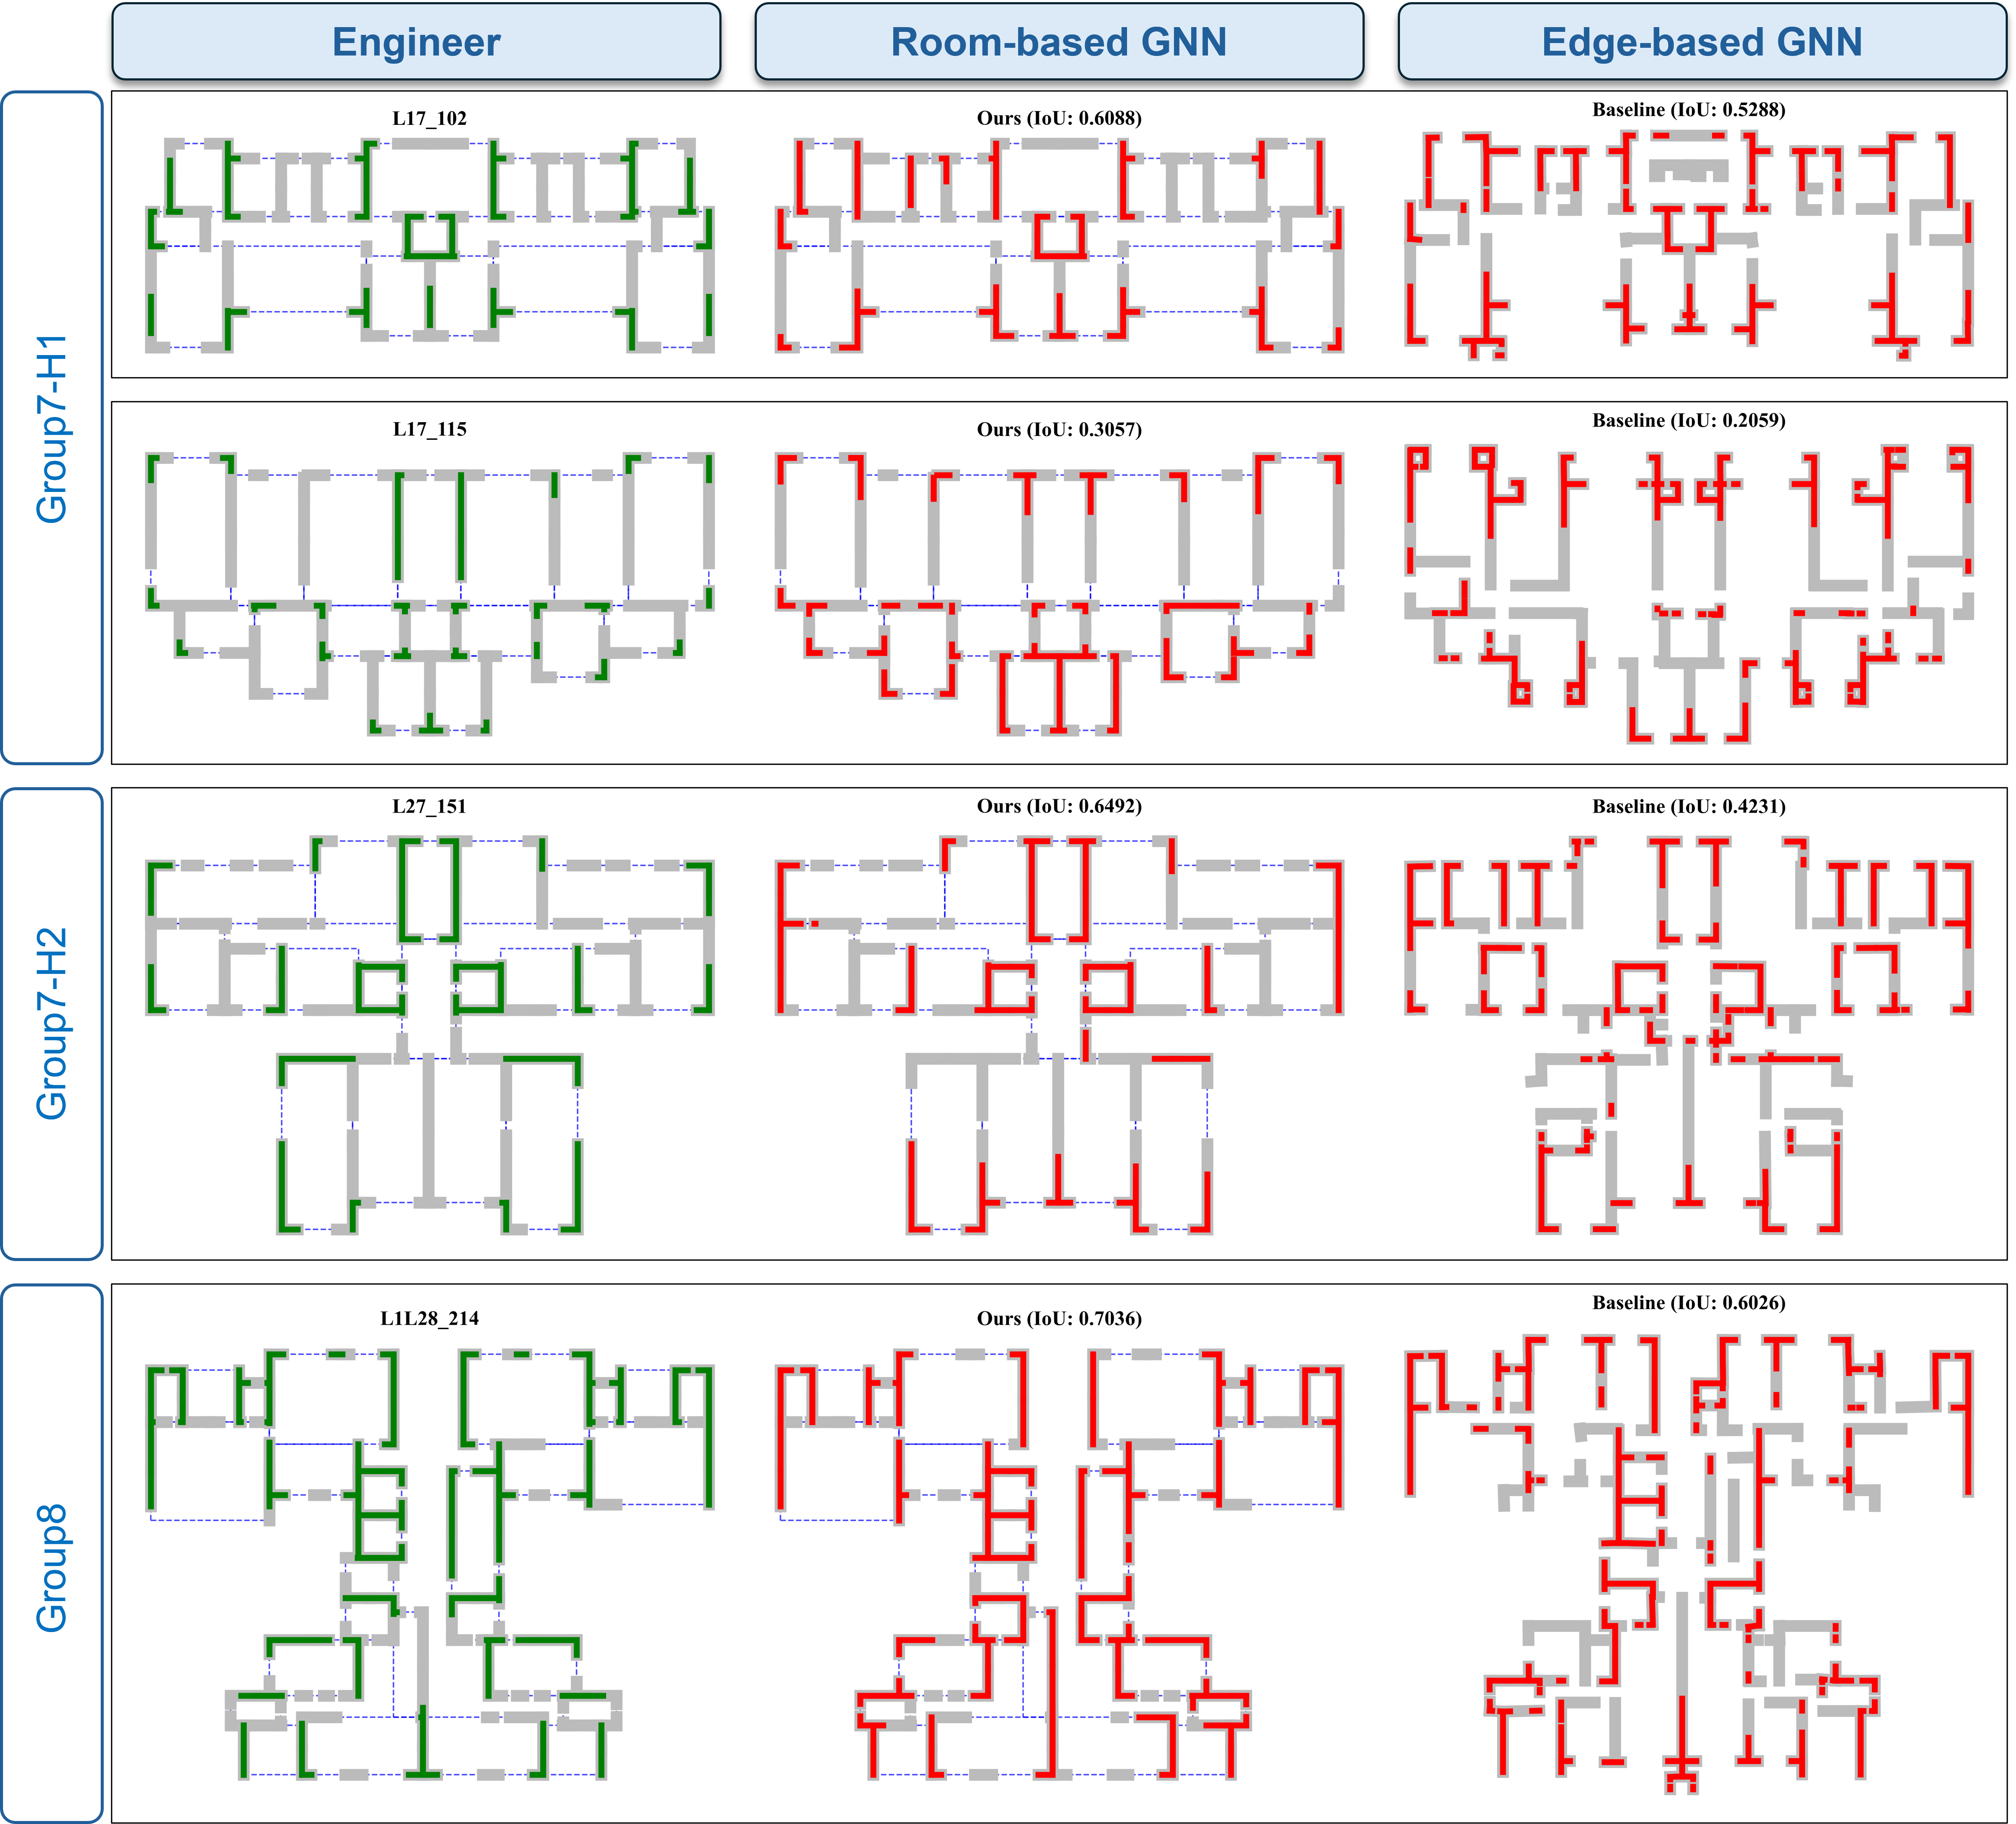
\includegraphics[width=0.9\textwidth]{figs/qual_comparison.png}
\caption{Qualitative comparison of predictions. Representative cases showing floor plan, ground truth, proposed method, and baseline. The proposed method produces fewer spurious segments and more coherent boundary-aligned predictions.}
\label{fig:qual_comparison}
\end{figure*}

\begin{figure*}[t]
\centering

\includegraphics[width=0.92\textwidth]{figs/boxplot.png}
\caption{Boxplot of CGS across 5-fold cross-validation for the full model and ablation variants, sorted by mean CGS. }
\label{fig:ablation_boxplot}
\end{figure*}

\begin{figure*}[t]
\centering
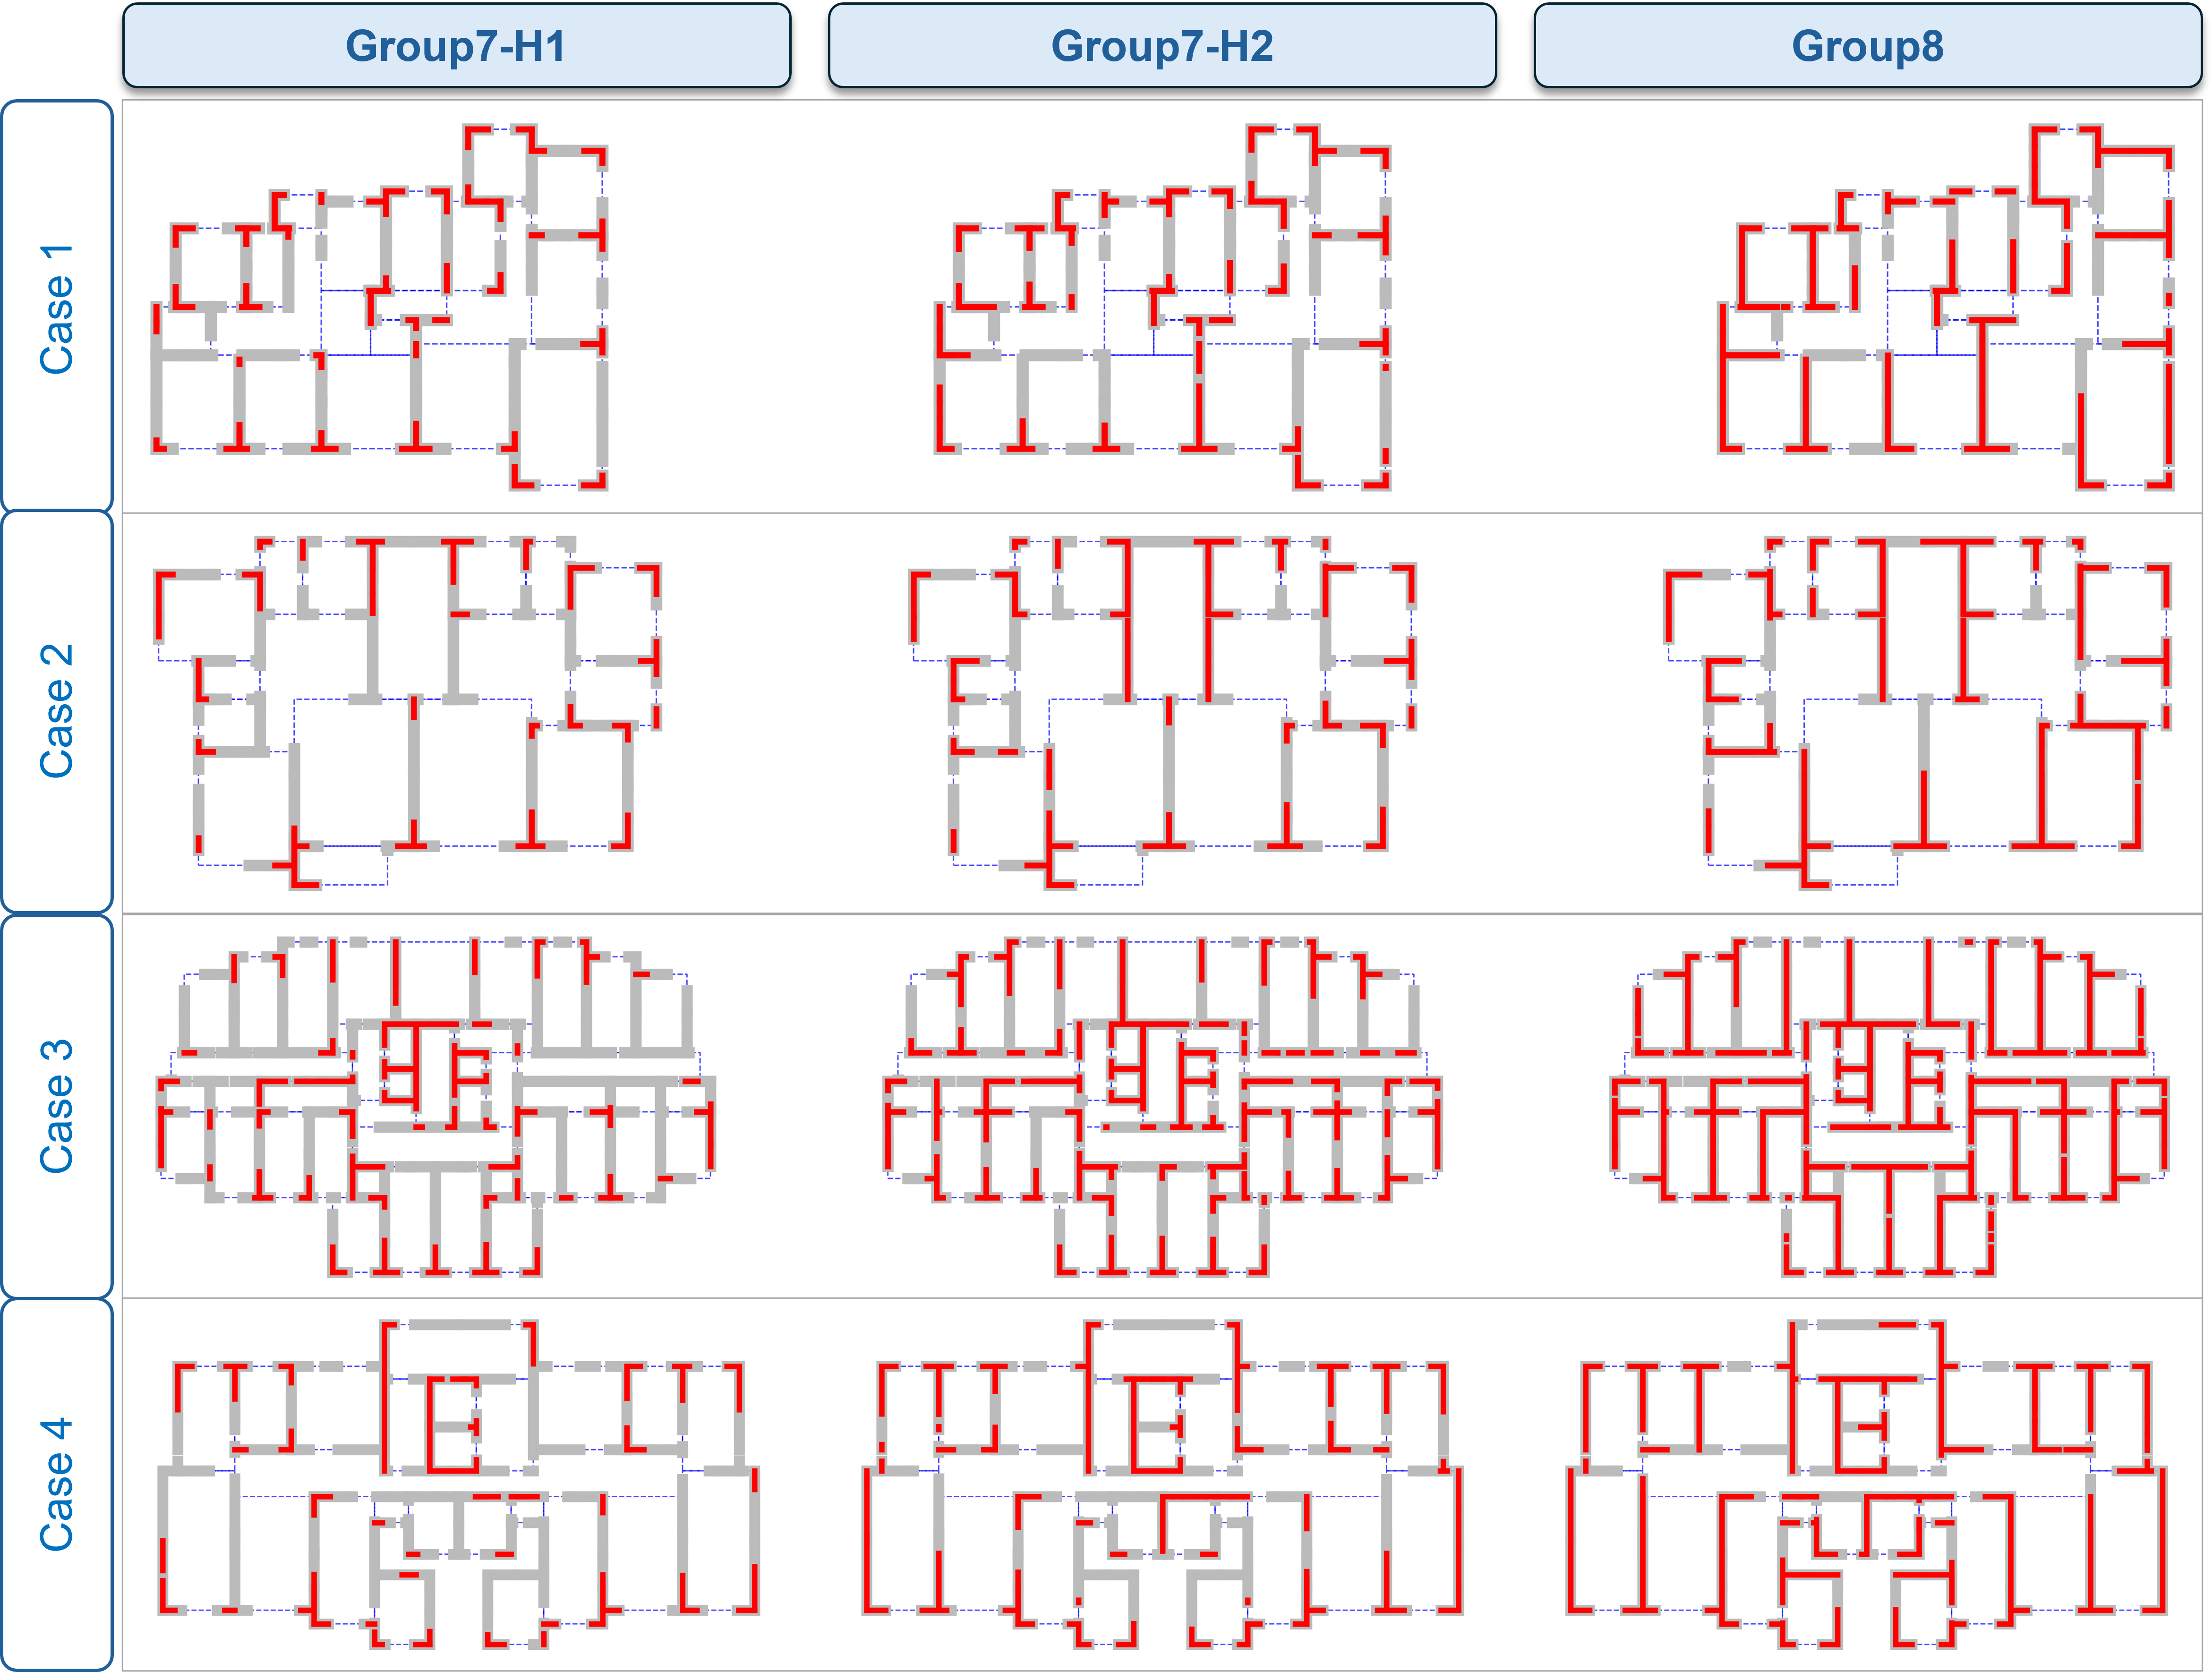
\includegraphics[width=0.9\textwidth]{figs/conditional_gen.png}
\caption{Conditional generation demonstration. For three representative floor plans, predictions under Low, Medium, and High conditions. Visual comparison shows progressive increase in wall density and coverage as condition severity increases.}
\label{fig:conditional_gen}
\end{figure*}

\begin{figure*}[t]
\centering
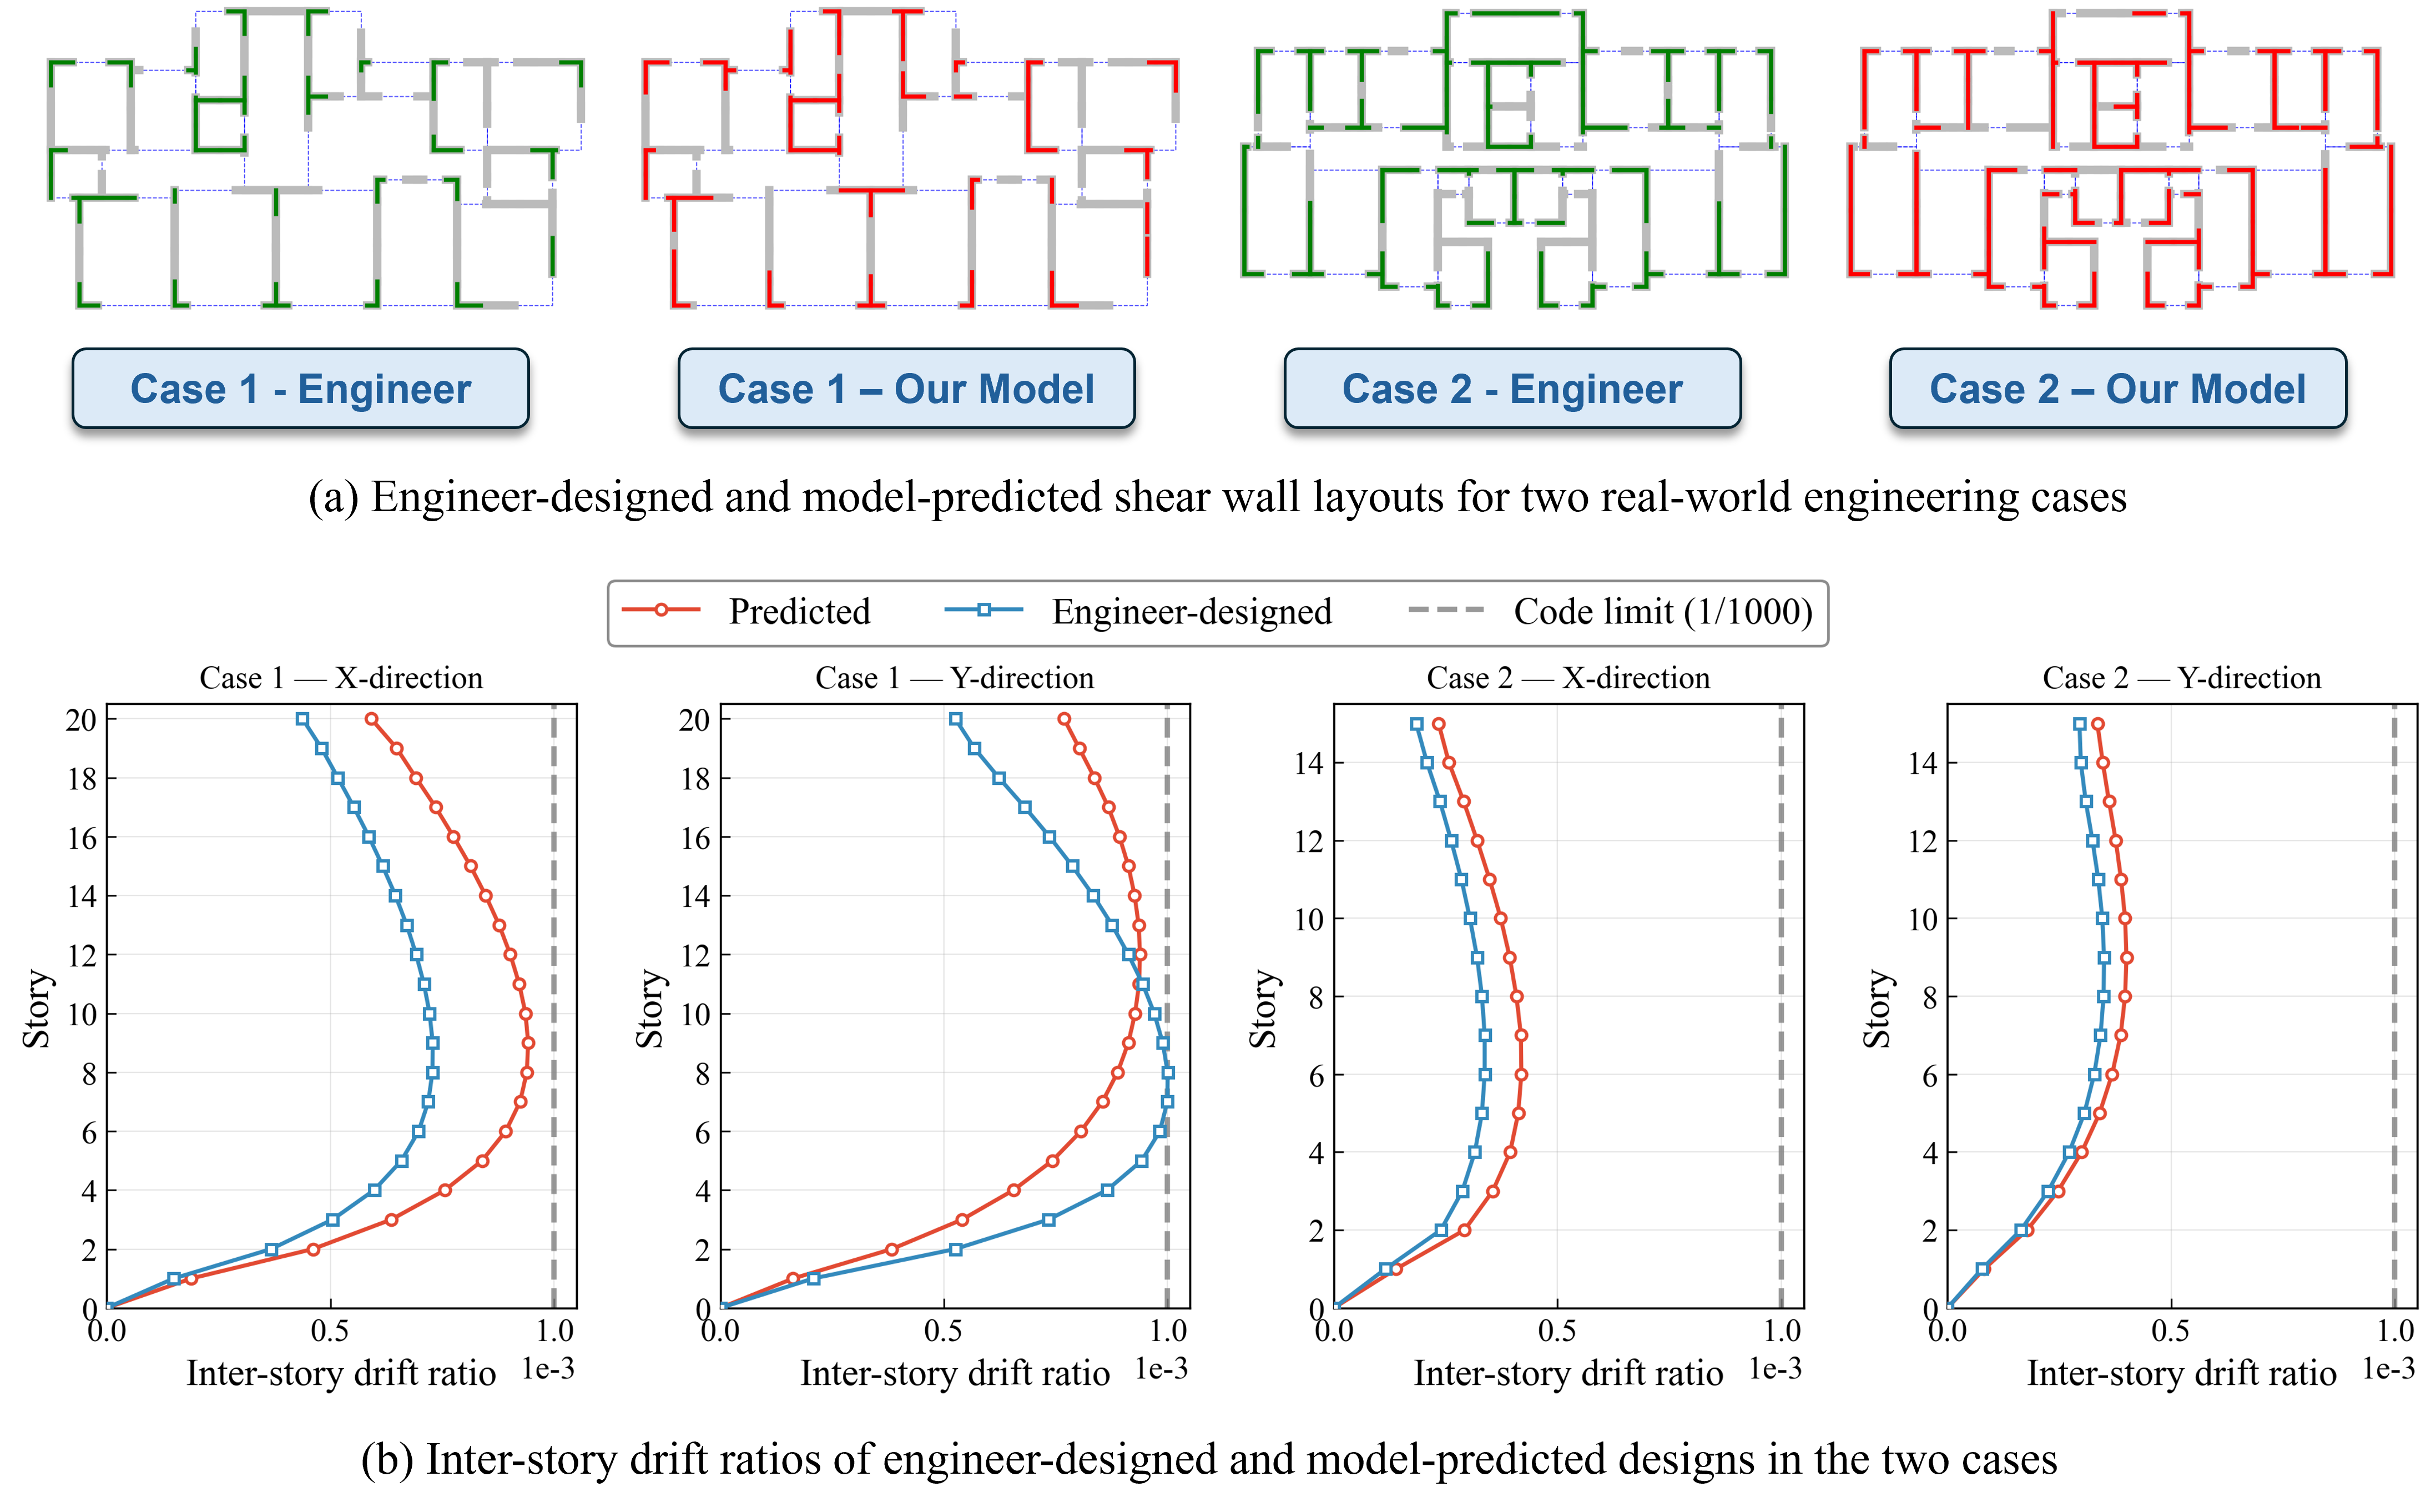
\includegraphics[width=\textwidth]{figs/case_study.png}
\caption{Engineering validation on two real projects. For each case, the model-predicted and engineer-designed schemes are compared in terms of inter-story drift ratios.}
\label{fig:case_study}
\end{figure*}

\begin{figure*}[t]
\centering
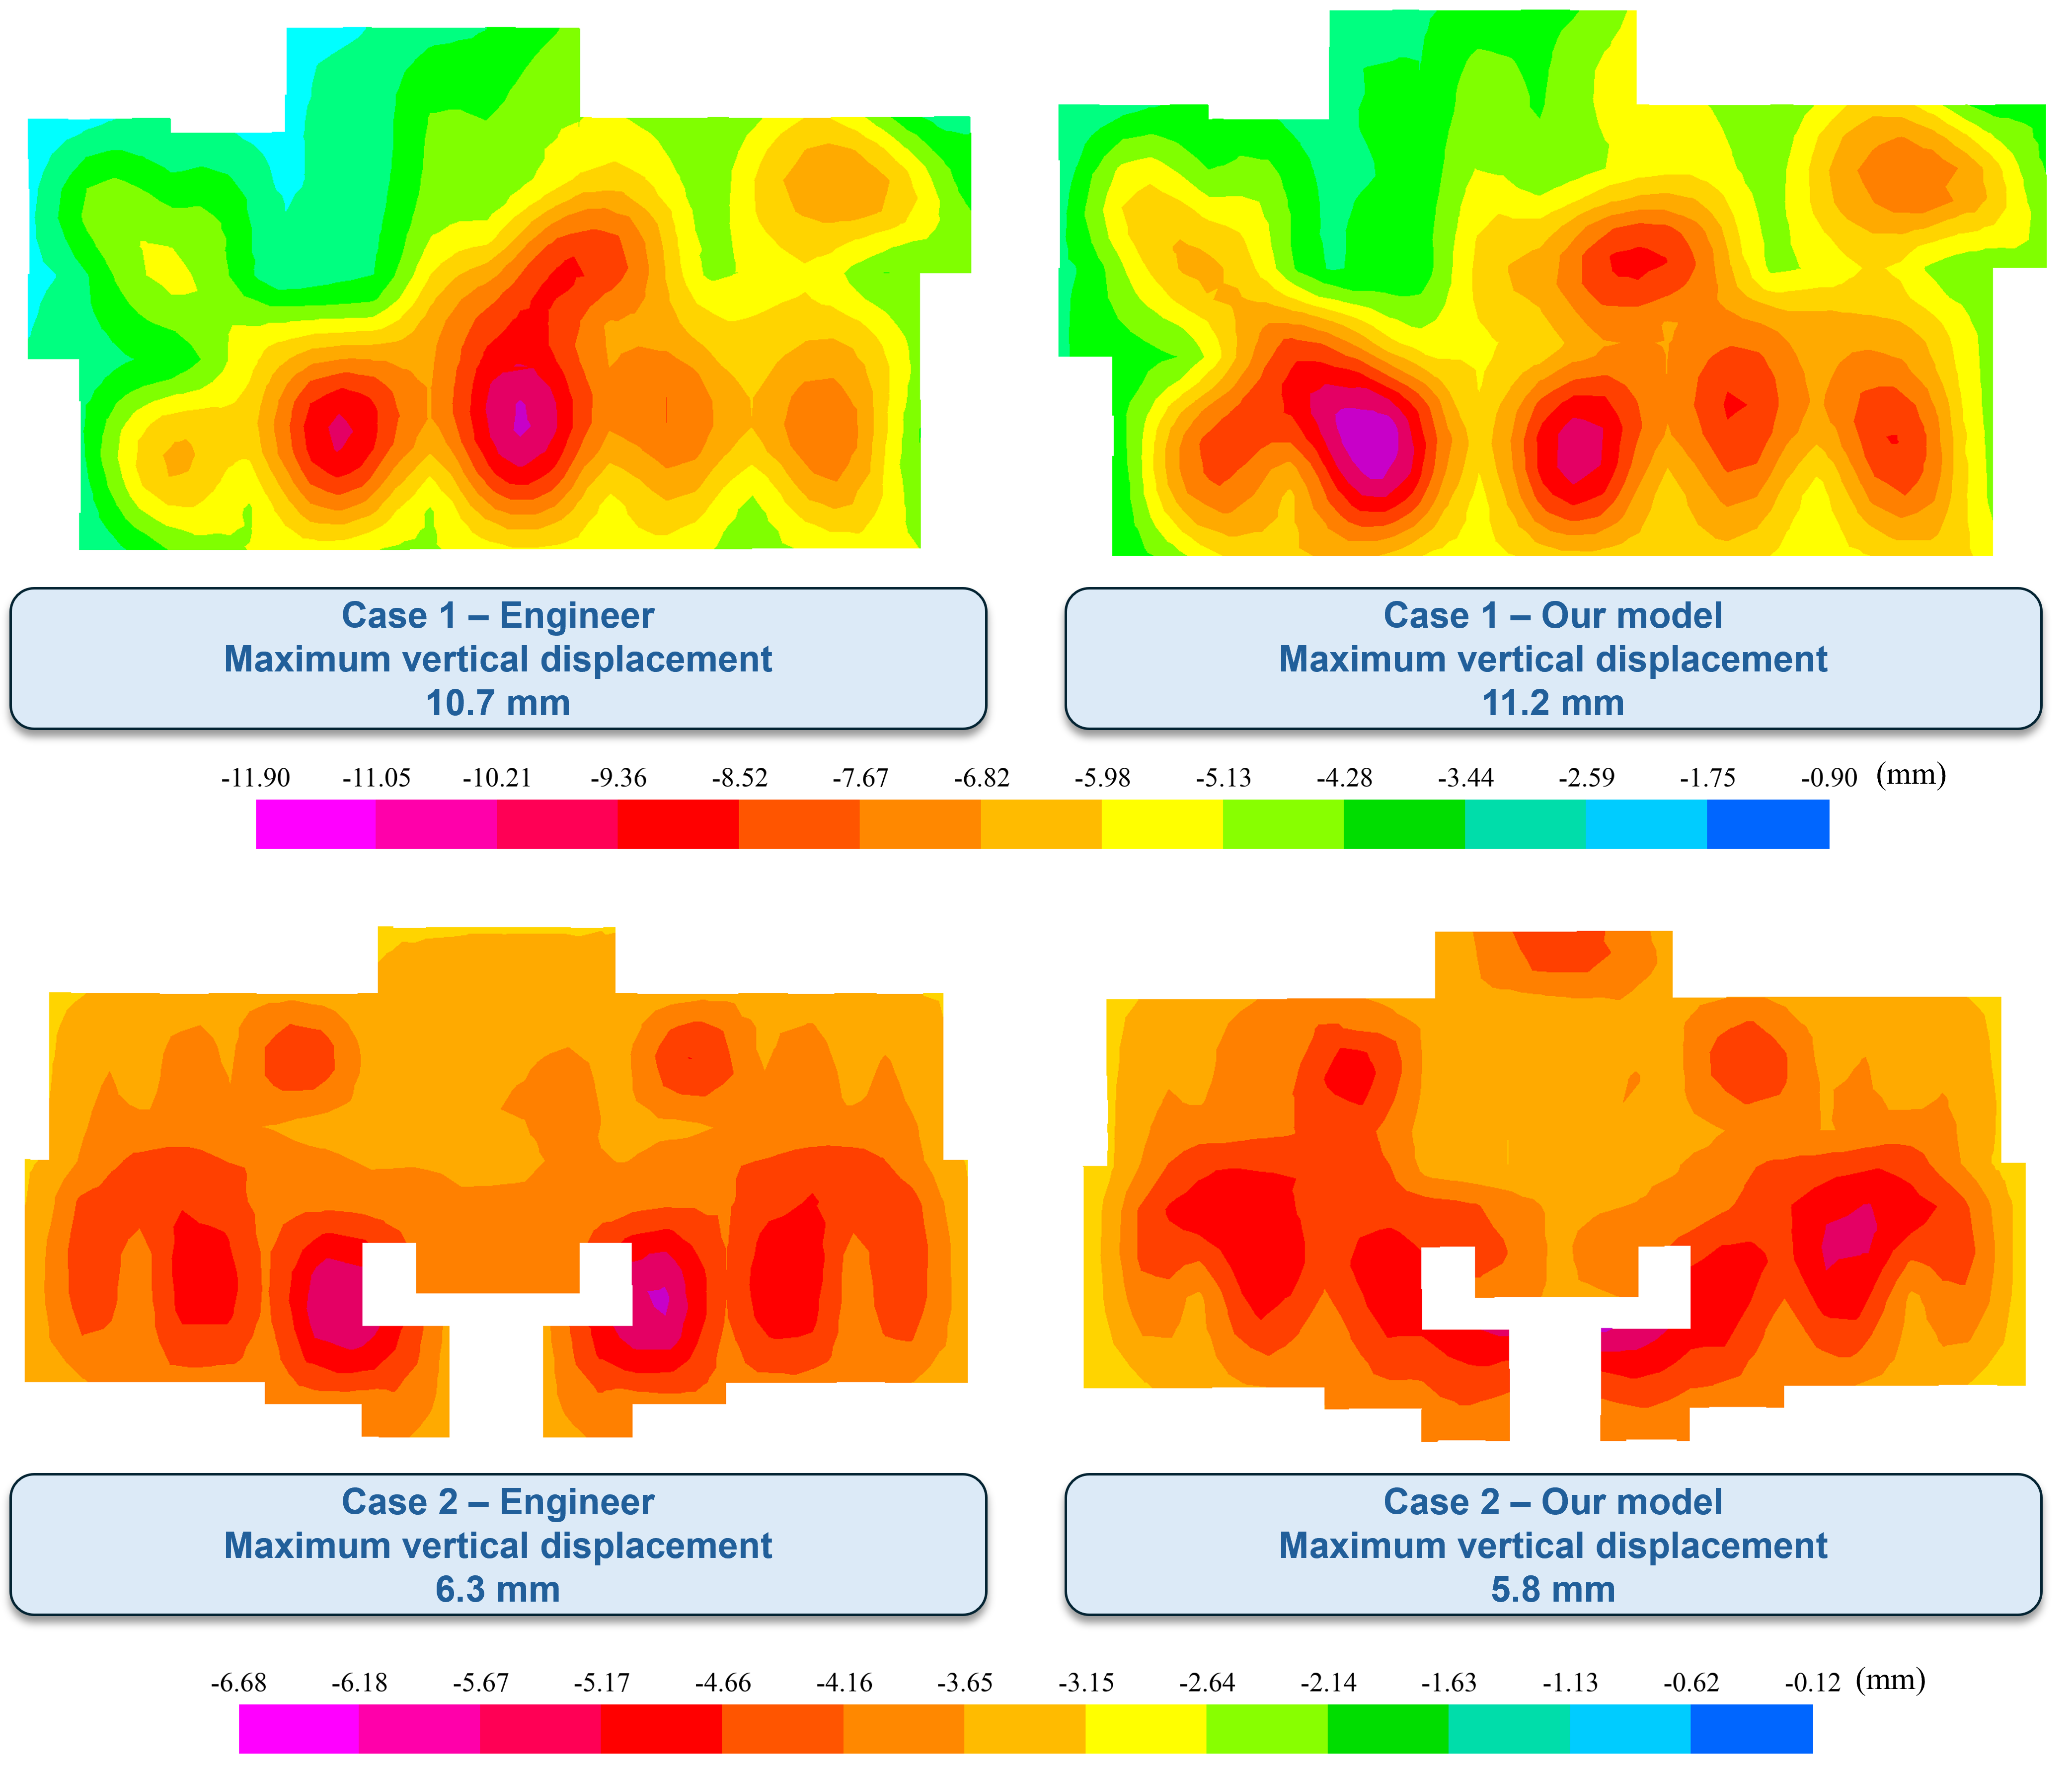
\includegraphics[width=0.85\textwidth]{figs/vertical_disp_cloud_diagram.png}
\caption{Vertical displacement cloud diagrams for Case 1 and Case 2, comparing the model-predicted scheme with the engineer-designed scheme.}
\label{fig:vertical_disp_cloud}
\end{figure*}

A dataset of high-rise residential floor plans is constructed from two sources: (i) the open-source shear-wall dataset reported by Liao et al. \cite{liaoAutomatedStructuralDesign2021a}, and (ii) additional engineering drawings provided by Tongji Architectural Design (Group) Co., Ltd. Each sample consists of an architectural floor plan and the corresponding shear-wall layout designed by licensed structural engineers. Raw CAD drawings are processed via contour extraction and semantic partitioning to identify functional rooms, and then converted into the room-based graph representation described in Section~\ref{subsec:room_graph}.

Following the condition taxonomy of Liao et al. \cite{zhaoIntelligentDesignShear2023b}, which accounts for the combined effects of seismic intensity and structural height, samples are categorized into three design-condition groups: Group7-H1, Group7-H2 and Group8. Specifically, the low-density group (Group7-H1) corresponds to seismic intensity 7 (PGA = 0.10g) and buildings with height $H \le 50$~m, while the medium-density group (Group7-H2) shares the same seismic intensity but covers higher buildings with $H > 50$~m. The high-density group (Group8) represents more demanding seismic settings with intensity 8 (PGA = 0.20g). The dataset statistics are summarized in Table~\ref{tab:dataset_stats}.



\subsubsection{Baselines}
\label{subsubsec:baselines}

To assess the impact of the proposed room-based representation, performance is compared against a representative edge-based GNN baseline consistent with prior literature. For the baseline, graphs are constructed using wall intersection points as nodes and wall segments as edges, and the model regresses continuous wall-coverage ratios for each segment, where two values are predicted to describe coverage measured from the two endpoints of the wall segment.

To isolate the effect of representation, the modeling and training configuration is kept comparable across methods: both use the same backbone family (GATv2), follow the same training schedule, apply the same data augmentation strategy, and adopt the same cross-validation protocol, with hyperparameters tuned on their respective validation sets. For the baseline, conditioning is incorporated by concatenating the design-condition embedding to both node and edge feature vectors, following the feature-concatenation strategy adopted in prior edge-based formulations. Because the open-source dataset does not provide continuous design parameters (e.g., PGA, site period, building height), the condition is represented as a one-hot encoded categorical variable corresponding to the three design groups, ensuring consistency with the available data.


\subsubsection{Implementation Details and Training Protocol}
\label{subsubsec:implementation}

The proposed room-based model uses a hidden dimension of 256 and a 32-dimensional condition embedding. The GNN encoder contains three GATv2 layers with four attention heads per layer and a dropout rate of 0.2. Models are trained with AdamW (learning rate $1\times 10^{-3}$, weight decay $1\times 10^{-4}$) for 100 epochs using a cosine-annealing learning-rate schedule with a 20-epoch warmup; the batch size is one graph per iteration. At inference time, a classification threshold of 0.5 is used for wall existence prediction, and a ratio threshold of 0.1 is applied when converting regressed segment ratios into final layout elements.

To improve generalization under limited data, standard geometric augmentations are applied to each training sample, including horizontal/vertical flips and rotations by 90$^{\circ}$, 180$^{\circ}$, and 270$^{\circ}$, with output labels transformed accordingly. To mitigate the imbalance among design conditions (Low:Medium:High = 33:52:58), weighted random sampling is adopted so that each epoch observes a more balanced mixture of conditions, following common practices for imbalanced deep learning problems \cite{johnsonSurveyDeepLearning2019}.

For robust reporting, 5-fold stratified cross-validation is employed with stratification by design condition; within each fold, 10\% of the training split is held out for validation and early stopping is applied with a patience of 20 epochs based on validation IoU. All experiments use a consistent preprocessing pipeline and the same train/test split within each fold \cite{Berrar_2019}.

All experiments are conducted on a workstation equipped with an Intel Core i7-12700F CPU, 32\,GB RAM, and an NVIDIA RTX 3060 GPU (12\,GB). The implementation is based on Python 3.12, PyTorch 2.5.1, and PyTorch Geometric 2.1.0.


\subsubsection{Evaluation Metrics}

\textbf{(1) Geometric accuracy.} For evaluation consistency across representations, predictions from both methods are rasterized into binary layout images and compared using Image IoU, which measures pixel-level overlap between predicted and reference shear-wall visualizations. Image IoU is used as the primary metric:
\[
\text{Image IoU}=\frac{|P\cap G|}{|P\cup G|}
\]
where $P$ and $G$ denote the predicted and ground-truth positive pixel sets, respectively. This image-based evaluation enables a representation-agnostic comparison across methods.

For the room-based method, a vector-level IoU is additionally reported on the 16-dimensional output parameterization to quantify parametric overlap without rasterization. Segment-level precision/recall/F1 are computed by thresholding predicted/ground-truth segment values at 0.01:
\begin{align*}
\text{Precision}&=\frac{TP}{TP+FP}, \quad
\text{Recall}=\frac{TP}{TP+FN}, \quad
\text{F1}=\frac{2PR}{P+R}.
\end{align*}
For correctly identified positive segments, MAE is used to evaluate the error of predicted length ratios \cite{Chai_2014}:
\[
\text{MAE}=\frac{1}{|S^+|}\sum_{(i,j)\in S^+}|\hat y_{ij}-y_{ij}|.
\]

\textbf{(2) Conditional generation.} Standard supervised metrics require matched ground-truth layouts and therefore cannot directly evaluate counterfactual conditions (e.g., generating a high-density layout for a plan labeled as low-density). To characterize conditional behavior across all conditions, the Conditional Generation Score (CGS) is defined as:
\[
\text{CGS}=w_1 S_{\text{den}}+w_2 S_{\text{IoU}}+w_3 S_{\text{uni}},
\quad w_1=w_2=w_3=\frac13.
\]
Here, $S_{\text{den}}$ measures compliance with target density statistics:
\[
S_{\text{den}}=1-\frac{|\bar\rho_{\text{pred}}-\bar\rho_{\text{target}}|}{\bar\rho_{\text{target}}}.
\]
$S_{\text{IoU}}$ corresponds to Image IoU when the generated condition matches the ground-truth label. $S_{\text{uni}}$ summarizes spatial rationality by combining global variation, local smoothness across adjacent rooms, and penalties for extreme outliers:
\[
S_{\text{uni}}=0.4\,(1-\text{CV})+0.4\,\text{Smoothness}+0.2\,(1-\text{OutlierRatio}).
\]

It should be noted that $S_{\text{den}}$ relies on target densities $\bar\rho_{\text{target}}$ empirically estimated from the training set for each design condition, and therefore reflects dataset-specific distributions rather than absolute engineering requirements. From a structural engineering perspective, higher seismic intensity and greater building height qualitatively necessitate increased lateral-load-resisting capacity, which typically manifests as higher shear-wall ratios \cite{GB500112010Code2016,qianDesignTallBuilding2018,zhangShearWallLayout2017}. The density compliance metric is thus intended to assess whether the model captures this qualitative trend---that generated layouts respond systematically to the specified condition---rather than to enforce a strict quantitative threshold. In practice, shear-wall ratios are determined through iterative structural analysis and code-checking rather than prescribed a priori, and the appropriate density for a given project depends on factors beyond the categorical condition labels available in the current dataset.



\subsection{Main Results}
\label{subsec:main_results}

Table~\ref{tab:main_results} reports the quantitative comparison between the proposed room-based GNN and the edge-based GNN baseline.



The proposed room-based representation yields higher Image IoU and F1 than the edge-based baseline under the same backbone family and training protocol. The largest gain is observed in precision (+17.5 pp), suggesting a marked reduction of false-positive wall predictions. This behavior is practically relevant because over-prediction can introduce unnecessary construction cost and increase the likelihood of conflicts with architectural constraints. In addition, the lower MAE/RMSE indicates improved accuracy in predicted wall-length ratios for correctly identified segments, which is consistent with the representation explicitly reasoning over complete room boundaries rather than isolated wall segments.

The qualitative comparisons in Fig.~\ref{fig:qual_comparison} provide visual evidence consistent with the quantitative results. Across different floor-plan cases, the room-based GNN generally produces wall layouts that are closer to the engineer-designed reference, with more coherent boundary-aligned wall placement and fewer spurious predictions. Correspondingly, the predicted layouts from the proposed method exhibit larger overlap with the ground truth, which is reflected in the higher Image IoU reported in Table~\ref{tab:main_results}.

By contrast, the edge-based baseline tends to generate more fragmented and isolated wall segments. These scattered predictions are especially visible in cases with complex room adjacencies, where local segment-level decisions do not fully capture the higher-level spatial organization of the floor plan. This qualitative failure mode is consistent with the lower representational level of the edge-based graph: because the model operates on individual wall primitives rather than room-level spatial units, it is more prone to producing locally plausible but globally incoherent wall fragments.



\subsubsection{Per-condition results}

To examine whether performance is consistent across design conditions, Table~\ref{tab:per_condition} reports Image IoU stratified by condition.

The proposed method outperforms the edge-based baseline in all three condition groups, indicating that the advantage of the room-level representation is not limited to a single density regime. The largest relative improvement is observed in the low-density group (Group7-H1, +34.14\%), where sparse wall distributions make false-positive predictions more detrimental to IoU. This result is consistent with the higher precision reported in the overall comparison and suggests that room-level boundary reasoning is particularly beneficial when valid wall segments are relatively few.

In absolute terms, the highest Image IoU is obtained in the high-density group (Group8, 0.6473), followed by the medium-density group (0.5975). One plausible explanation is the imbalance of the training data across categories: the three groups are distributed as 33:52:58, so the high-density category is represented by the largest number of samples. This gives the model more opportunities to learn stable category-specific patterns for Group8. In addition, denser layouts provide stronger geometric signals and more continuous boundary-aligned wall patterns, which are easier for both models to learn than sparse layouts. Even under these more favorable settings, however, the proposed method still maintains clear gains over the baseline, with improvements of 17.20\% and 15.62\% in the high- and medium-density groups, respectively.

The standard deviations also provide useful insight into robustness. Performance in the medium- and high-density groups is relatively stable across folds, whereas the low-density group shows larger variance for both methods. This suggests that sparse-layout cases are inherently more sensitive to sample composition and prediction thresholding, and that the smaller sample size of the low-density group further increases uncertainty. Nevertheless, the proposed method consistently preserves a margin over the baseline in every condition group, supporting the claim that the room-based formulation improves both average accuracy and cross-condition robustness.


\subsection{Ablation Studies}
\label{subsec:ablation}

\newcolumntype{Y}{>{\centering\arraybackslash}X}

\begin{table*}[t]
\centering
\caption{Ablation Study Results}
\small
\label{tab:ablation}
\begin{tabularx}{\textwidth}{l *{5}{Y}}
\toprule
Configuration & CGS  & Density ($S_{den}$)  & IoU ($S_{IoU}$)  & Uniformity ($S_{uni}$)  & Score$_{\text{DC}}$ \\
\midrule
Full Model & 0.679 & 0.750 & 0.541 & 0.812 & 0.413 \\
\midrule
\textit{Conditioning Mechanism} & & & & & \\
w/o conditioning & 0.531 (-0.148) & 0.384 & 0.535 & 0.816 & 0.388 \\
w/o FiLM (concat early) & 0.672 (-0.007) & 0.751 & 0.507 & 0.842 & 0.349 \\
w/o FiLM (concat late) & 0.670 (-0.009) & 0.756 & 0.496 & 0.845 & 0.334 \\
\midrule
\textit{Loss Functions} & & & & & \\
w/o density loss & 0.621 (-0.058) & 0.607 & 0.542 & 0.805 & 0.427 \\
w/o IoU loss & 0.644 (-0.035) & 0.772 & 0.366 & 0.945 & 0.2763 \\
w/o consistency loss & 0.674 (-0.005) & 0.749 & 0.519 & 0.835 & 0.359 \\
w/o all auxiliary losses & 0.574 (-0.105) & 0.616 & 0.340 & 0.958 & 0.355 \\
\midrule
\textit{Training Strategy} & & & & & \\
w/o dual-stream & 0.666 (-0.013) & 0.730 & 0.523 & 0.825 & 0.394 \\
w/o warmup & 0.636 (-0.043) & 0.700 & 0.462 & 0.853 & 0.299 \\
w/o augmentation & 0.653 (-0.026) & 0.742 & 0.462 & 0.859 & 0.277 \\
\midrule
\textit{GNN Backbone} & & & & & \\
GCN & 0.664 (-0.015) & 0.745 & 0.482 & 0.865 & 0.292 \\
GraphSAGE & 0.664 (-0.015) & 0.727 & 0.513 & 0.838 & 0.349 \\
GIN & 0.666 (-0.013) & 0.753 & 0.480 & 0.866 & 0.312 \\
\bottomrule
\end{tabularx}
\end{table*}




Ablation experiments were conducted to quantify the contribution of each component. Table~\ref{tab:ablation} summarizes results using the Conditional Generation Score (CGS) and its sub-metrics.

Fig.~\ref{fig:ablation_boxplot} provides a complementary view of the same ablation results by visualizing the fold-wise CGS distribution of each variant. The most pronounced degradation occurs when conditioning is removed, where the CGS distribution shifts downward relative to the full model. This confirms that the conditioning mechanism is the primary basis for controllable generation rather than a marginal refinement.

The conditioning module accounts for the largest change in controllability-related performance. Removing conditioning reduces CGS by 0.148, driven primarily by a sharp drop in density consistency ($S_{den}$: 0.750 $\rightarrow$ 0.384), indicating that outputs become less responsive to the specified design condition. Among alternative injection strategies, FiLM yields small but consistent gains over early and late feature concatenation.

Loss-term ablations show complementary roles. The density loss most strongly affects conditional compliance (CGS -0.058 when removed), primarily through reduced $S_{den}$, indicating that layout-density regulation contributes substantially to the overall CGS. The IoU loss contributes to geometric fidelity ($S_{IoU}$: 0.541 $\rightarrow$ 0.366 when removed) while increasing uniformity ($S_{uni}$: 0.812 $\rightarrow$ 0.945), suggesting a trade-off between boundary accuracy and distribution smoothness under the current metric definition. The consistency loss produces a smaller but measurable effect (CGS -0.005), and removing all auxiliary losses leads to a substantial overall degradation (CGS -0.105).

Training-related components have moderate but non-negligible impacts. Eliminating the dual-stream strategy decreases CGS by 0.013, with the main change in $S_{den}$, consistent with improved condition sensitivity. Warmup contributes to optimization stability (CGS -0.043 without warmup). Data augmentation primarily benefits IoU (0.541 $\rightarrow$ 0.462 without augmentation). From the boxplot, both the `w/o augmentation` and `w/o warmup` variants exhibit visibly larger spread and more unstable fold-wise behavior than the full model, indicating that these components mainly improve robustness and consistency rather than only the best-case score.

For the GNN backbone, GATv2 achieves the best overall CGS; replacing it with GCN, GraphSAGE, or GIN results in consistent but modest decreases (approximately 0.013--0.015 in CGS). The small gaps among these backbones, together with the limited differences between early and late concatenation variants, suggest that the overall performance is driven more strongly by the representation, conditioning objective, and loss design than by a single specific graph convolution operator.

Finally, the full model not only attains the highest median CGS but also shows a comparatively compact distribution across folds. This indicates that the proposed combination of room-level representation, conditioning, and auxiliary objectives improves both average performance and training stability.



\subsection{Conditional Generation Analysis}
\label{subsec:conditional_analysis}

The ability to generate condition-dependent layouts is evaluated by applying all three condition inputs to the same set of floor plans.

\begin{table*}[t]
\centering
\caption{Density Statistics by Condition}
\label{tab:density_stats}
\begin{tabularx}{\textwidth}{XXXX}
\toprule
Input Condition & Target Density & Generated Density \newline (Mean $\pm$ Std) & Density Error(\%) \\
\midrule
Low (0) & 3.62 $\pm$ 1.02 & 3.42 $\pm$ 0.69 & 5.6 \\
Medium (1) & 4.89 $\pm$ 0.82 & 5.14 $\pm$ 1.01 & 5.0 \\
High (2) & 8.71 $\pm$ 1.04 & 7.96 $\pm$ 0.93 & 8.6 \\
\bottomrule
\end{tabularx}
\end{table*}

Fig.~\ref{fig:conditional_gen} shows that predicted layouts vary systematically across conditions, with denser wall coverage under more demanding settings. Table~\ref{tab:density_stats} further reports the corresponding density statistics. Density errors remain within 8.6\% of target values, indicating condition-responsive generation under the current definition of density and evaluation protocol.



\subsection{Case Study: Engineering Validation}
\label{subsec:case_study}

To further verify engineering feasibility, two real projects outside the training set are selected for finite-element validation: Case 1 (story height 3.3\,m, 20 stories, seismic intensity 7) and Case 2 (story height 3.0\,m, 15 stories, seismic intensity 8). For each project, two structural schemes are analyzed under the same modeling assumptions: (i) the layout predicted by the proposed model and (ii) the reference layout designed by licensed engineers.

For both cases, room-based predictions are first converted into vector structural members and then imported into structural analysis software to build FE models. Response-spectrum analysis is conducted to obtain inter-story drift ratios and displacement responses, consistent with standard seismic evaluation practice for building structures \cite{GB500112010Code2016,qianDesignTallBuilding2018}. The comparisons focus on two practical indicators: the story-wise drift ratio distribution and the maximum vertical displacement of each floor.





As shown in Fig.~\ref{fig:case_study}, the predicted schemes in both cases exhibit drift-ratio profiles close to those of the engineer-designed schemes, and all story drift ratios are below the code limit of $1/1000$ \cite{GB500112010Code2016}. Fig.~\ref{fig:vertical_disp_cloud} further shows that the vertical-displacement cloud patterns are highly consistent between the two schemes, with only small differences in maximum floor vertical displacement. These results suggest that the generated layouts preserve key global stiffness characteristics in practical FE evaluation and support the applicability of the proposed method in preliminary structural scheme generation.
